% Provenance (never printed): see sources/outline_sources.md (Year 3:
% fractionation and Rayleigh distillation in the water cycle;
% palaeothermometry; carbon and sulfur isotopes). Brief:
% sources/book5/BRIEFS.md, ch. 14. Curves from figdata/bachelor-3/
% rayleigh_distillation.py, lr04_d18o.py, carbon_mass_balance.py. Exercise
% and problem values in the Book 5 scratch calculator calc/ch14.py. Dome Ilse,
% its traverse and the marine core are invented.
\chapter{الجيوكيمياء النظيرية المستقرّة}\label{ch:b3:stable-isotopes}

يُعدّ الثلجُ المتساقط على القباب المرتفعة للغطاء الجليدي في شرق القارة القطبية الجنوبية
من أخفّ المياه على سطح الأرض. غادرت كلّ جزيئة من جزيئاته المحيطَ بخارًا،
وفي طريقه نحو الداخل فقد الهواء معظم مائه ثلجًا، والجزيئات الثقيلة
أولًا. فما يبقى عند الوصول يتوقّف على مقدار ما فُقد، والمقدار نفسه يتوقّف على
مدى برودة الهواء. ومن ثمّ فإنّ عمود الجليد مقياسٌ حراري، وقوقعةُ الكالسيت مقياسٌ آخر،
وكربونُ الحجر الجيري سجلٌّ لما دفنه
الغلاف الحيوي. يشتقّ هذا الفصلُ القوانينَ الكامنةَ وراء هذه السجلّات
ويقرؤها.

\begin{recall}
قيمة $\delta$، ومعامل التجزّؤ $\alpha$، وتأثيرات النظائر التوازنية والحركية، واردةٌ في
المجلّدات الجامعية لكتب الكيمياء. أمّا المعايير المرجعية
VSMOW و VPDB وخطّ المياه الجوية واردةٌ في
مجلد السنة الثانية، في فصله عن الجيوكيمياء النظيرية؛
قانون تجزّؤ رايلي للعناصر النزرة في فصله عن التمايز الصهاري؛
والبدائل المناخية، وأثر حجم الجليد، ومقياس الحرارة Mg/Ca
في فصله عن أرشيفات المناخ والبدائل؛ والحدّ الحراري
الأقصى بين الباليوسين والإيوسين في فصله عن المناخ عبر
الزمن الجيولوجي؛ وحدث الأكسدة العظيم في فصله عن الأرض في ما قبل الكمبري.
يقع البناء الضوئي والاختزال البكتيري للكبريتات في كتب الأحياء.
\end{recall}

\section{التجزّؤ بين طورين}\label{sec:b3:stable-isotopes:fractionation}

للطورين A و B في التوازن النظيري، $\alpha_{A-B} = R_A/R_B =
(1000 + \delta_A)/(1000 + \delta_B)$، مع النسب $R$ للنظير الثقيل إلى
النظير الخفيف. لبخار الماء والماء السائل $\alpha = 1.0098$ للأكسجين-18
و$1.084$ للدوتيريوم عند \qty{20}{\celsius}، و$1.0117$ و$1.111$ عند
\qty{0}{\celsius}؛ والجليد والماء عند \qty{0}{\celsius}، $1.0035$ و$1.0208$.
الطور الأثقل هو الأكثر تكثّفًا دائمًا، ويزداد التجزّؤ
كلّما انخفضت درجة الحرارة.
% ledger: kc98:alpha, kc98:standards

\begin{definition}[الفرق النظائري]\label{def:b3:stable-isotopes:big-delta}
\emph{الفرق النظائري}\index{الفرق النظائري (دلتا الكبيرة)}
بين طورين هو $\Delta_{A-B} = \delta_A - \delta_B$، مقدّرًا بالألف.
\end{definition}

\begin{proposition}[الفرق النظائري ومعامل التجزّؤ]
\label{prop:b3:stable-isotopes:big-delta}
عندما يكون $\alpha$ قريبًا من 1 وقيم $\delta$ صغيرة،
\[
\Delta_{A-B} \approx 1000\ln\alpha_{A-B} \approx 1000(\alpha_{A-B} - 1).
\]
\end{proposition}

\begin{proof}
$1000\ln\alpha = 1000\ln(1 + \delta_A/1000) - 1000\ln(1 + \delta_B/1000)$،
و$1000\ln(1 + x/1000) = x - x^2/2000 + \dots$، ومنه $1000\ln\alpha = \delta_A -
\delta_B - (\delta_A^2 - \delta_B^2)/2000 + \dots$. وأخيرًا $\ln\alpha \approx
\alpha - 1$ عندما يكون $\alpha$ قريبًا من 1.
\end{proof}

الخطأ هو $(\delta_A^2 - \delta_B^2)/2000$: جزءٌ من الألف عند
قيم المحيط، وقرابة واحد في الألف بين المحيط والثلج الخفيف
للجليد القطبي.
والكمّية $1000\ln\alpha$ هي التي تربطها النظرية بدرجة الحرارة: فهي
تتغيّر تقريبًا بما يناسب $1/T^2$ عند درجة الحرارة المرتفعة، وبما يناسب $1/T$ عند المنخفضة،
وتُكتب المعايرات بهذه الصيغة. فمثلًا، للجليد والبخار،
\[
\ln\alpha^{18}_{\mathrm{ice-v}} = \frac{11.839}{T} - 0.028224, \qquad
\ln\alpha^{\mathrm D}_{\mathrm{ice-v}} = \frac{16288}{T^2} - 0.0934,
\]
حيث $T$ بالكلفن.
% ledger: gkinis14:alpha-ice, kc98:standards

\begin{definition}[التجزّؤ المعتمد على الكتلة والتجزّؤ المستقل عن الكتلة]\label{def:b3:stable-isotopes:mif}
العنصر الذي له ثلاثة نظائر أو أكثر يكون له \emph{التجزّؤ المعتمد
على الكتلة}\index{التجزّؤ المعتمد على الكتلة} عندما تكون تجزّؤاتُ
نِسَب نظائره متناسبةً مع فروق كتلها، كما تحدّدها
الكتلُ؛ وإلّا فله \emph{التجزّؤ المستقل
عن الكتلة}\index{التجزّؤ المستقل عن الكتلة}، ويُقاس بمقدار انحرافه
عن خط التجزّؤ المعتمد على الكتلة، مثل $\Delta^{33}\mathrm S = \delta^{33}\mathrm S
- 0.515\,\delta^{34}\mathrm S$.
\end{definition}

في حالة الأكسجين يبلغ تجزّؤ $^{17}\mathrm O/^{16}\mathrm O$ نحو 0.52 مرّة من
تجزّؤ $^{18}\mathrm O/^{16}\mathrm O$، وهي نسبة قريبة من نسبة فروق الكتل، أي 1 إلى 2؛
وبالنسبة للكبريت، $\delta^{33}\mathrm S = 0.515\,\delta^{34}\mathrm S$. \omterm{def:b3:stable-isotopes:mif}{والتجزّؤ
المستقل عن الكتلة} نادرٌ: يوجد في النيازك، وفي أوزون الستراتوسفير،
وفي كبريت الأركي.
% ledger: white13c9:mdf, white13c9:s-mif

\section{تقطير رايلي في الدورة المائية}\label{sec:b3:stable-isotopes:rayleigh}

تُكوّن الكتلة الهوائية المتبرّدة قطيرات سحابية أو بلورات ثلجية تهبط
وتغادر. يكون كلّ مكثّف أغنى بالنظائر الثقيلة من البخار، فيصير
البخار المتبقّي أخفّ، ويكون المكثّف التالي، في التوازن معه، أخفّ
أيضًا.

\begin{proposition}[تقطير رايلي]\label{prop:b3:stable-isotopes:rayleigh-distillation}
لنفترض خزّان بخار يفقد مياهه بمكثّفات، تُزال كلّ منها ما إن
يتكوّن في التوازن مع البخار. إذا كان $f$ هو كسر البخار المتبقّي
و$\alpha$ معامل تجزّؤ المكثّف--البخار، فإنّ
تخضع نسبة البخار للعلاقة $\mathrm d\ln R_v = (\alpha - 1)\,\mathrm d\ln f$. وإذا
كان $\alpha$ ثابتًا فهذا هو \emph{تقطير
رايلي}\index{تقطير رايلي}:
\[
\frac{R_v}{R_{v,0}} = f^{\,\alpha - 1}, \qquad
\delta_v = (1000 + \delta_{v,0})\,f^{\,\alpha - 1} - 1000,
\]
ويكون المكثّف المتكوّن عند $f$ قيمته $\delta_c = \alpha(1000 + \delta_v) - 1000$.
\end{proposition}

\begin{proof}
ليكن $N$ عدد جزيئات البخار (معظمها خفيف) و$N R_v$
عدد الجزيئات الثقيلة فيه. إزالة $\mathrm dN < 0$ جزيئًا من المكثّف
تُزيل $\alpha R_v\,\mathrm dN$ جزيئًا ثقيلًا: $\mathrm d(NR_v) = \alpha
R_v\,\mathrm dN$. ومنه $N\,\mathrm dR_v = (\alpha - 1)R_v\,\mathrm dN$، وهذا هو
القانون التفاضلي مع $f = N/N_0$. وعند ثبات $\alpha$ يُكامَل إلى
قانون القوّة.
\end{proof}

عندما يعتمد $\alpha$ على درجة الحرارة، فإنّ $\ln(R_v/R_{v,0}) = \int(\alpha - 1)\,
\mathrm d\ln f$ على طول المسار. أمّا كتلة هوائية مبرّدة عند ضغط ثابت،
فإنّ كمية البخار التي يمكنها حملها تتحدّد بضغط التشبّع، ومنه $f =
e_s(T)/e_s(T_0)$، وهذا ما يعطيه منحنى التسامي للجليد أدنى
\qty{0}{\celsius}. يُكامِل الشكل أدناه القانون لكتلة هوائية يبدأ بخارها عند
\qty{0}{\celsius} وقيمة مفترَضة $\delta^{18}\mathrm O = -20$
و$\delta\mathrm D = \qty{-150}{\permil}$. البخار الحقيقي فوق المحيط أخفّ
مما يجعله التوازن مع ماء البحر، نحو $-13$ بدلًا من
\qty{-9}{\permil} في الأكسجين-18، لأنّ التبخّر حركي جزئيًا.
% ledger: iapws:melt-subl, gkinis14:alpha-ice, white13c9:rayleigh

\begin{definition}[فائض الدوتيريوم]\label{def:b3:stable-isotopes:d-excess}
\emph{فائض الدوتيريوم}\index{فائض الدوتيريوم} لعيّنة ماء هو $d =
\delta\mathrm D - 8\,\delta^{18}\mathrm O$، بالألف.
\end{definition}

يقع هطول الأمطار من قارات نصف الكرة الشمالي على الخطّ
$\delta\mathrm D = 8.0\,\delta^{18}\mathrm O + 10$، \omterm{def:b3:stable-isotopes:d-excess}{وفائض الدوتيريوم} فيه نحو
\qty{10}{\permil}. والميل 8 قريب من نسبة التجزّؤات التوازنية للنظيرين
في التكاثف. والفائض 10، لا 0، يسجّل التبخّر الحركي من المحيط،
ويقيس فائض أيّ عيّنة
مدى بُعد تبخّر مائها عن التوازن.
% ledger: dansgaard64:effects, kc98:mwl

\begin{omfigure}
\begin{tikzpicture}
\begin{groupplot}[group style={group size=2 by 1, horizontal sep=1.6cm},
  omrecord, width=0.47\linewidth, height=0.42\linewidth, title style={font=\small},
  tick label style={font=\scriptsize}, label style={font=\small},
  legend style={font=\scriptsize, legend cell align=left}]
\nextgroupplot[title={(أ) على طول مسار التبريد},
  xlabel={درجة حرارة التكاثف \babelsublr{(\unit{\celsius})}}, ylabel={\mbox{\textdir TLT $\delta^{18}\mathrm O$ (\unit{\permil})}},
  xmin=-55, xmax=0, ymin=-130, ymax=0, x dir=reverse,
  legend style={at={(0.03,0.03)}, anchor=south west}]
% computed in figdata/bachelor-3/rayleigh_distillation.py
\addplot[omDef, thick, densely dashed] table[x=t, y=d18v] {figdata/out/bachelor-3-rayleigh_distillation-curve.dat};
\addlegendentry{بخار}
\addplot[omDef, thick] table[x=t, y=d18s] {figdata/out/bachelor-3-rayleigh_distillation-curve.dat};
\addlegendentry{ثلج}
\addplot[red!70!black, only marks, mark=*, mark size=1.6pt] table[x=t, y=d18s] {figdata/out/bachelor-3-rayleigh_distillation-stations.dat};
\addlegendentry{المحطّات}
\nextgroupplot[title={(ب) الثلج على مخطّط $\delta\mathrm D$--$\delta^{18}\mathrm O$},
  xlabel={\mbox{\textdir TLT $\delta^{18}\mathrm O$ (\unit{\permil})}}, ylabel={\mbox{\textdir TLT $\delta\mathrm D$ (\unit{\permil})}},
  xmin=-110, xmax=0, ymin=-700, ymax=0,
  legend style={at={(0.97,0.03)}, anchor=south east}]
\addplot[omDef, thick] table[x=d18s, y=dDs] {figdata/out/bachelor-3-rayleigh_distillation-curve.dat};
\addlegendentry{الثلج النموذجي}
\addplot[black, densely dotted, domain=-110:0, samples=2] {8*x + 10};
\addlegendentry{$\delta\mathrm D = 8\,\delta^{18}\mathrm O + 10$}
\addplot[red!70!black, only marks, mark=*, mark size=1.6pt, forget plot] table[x=d18s, y=dDs] {figdata/out/bachelor-3-rayleigh_distillation-stations.dat};
\end{groupplot}
\end{tikzpicture}

\par\smallskip{\small \omterm{prop:b3:stable-isotopes:rayleigh-distillation}{تقطير رايلي} لكتلة هوائية مبرّدة عند ضغط ثابت
ابتداءً من \qty{0}{\celsius}، ومعاملات تجزّؤ الجليد--البخار
وكسر البخار المتبقّي مقروءَين من منحنى التسامي للجليد. (أ) البخار
(المتقطّع) والثلج (المتّصل) يزدادان خفّةً بتسارع متزايد؛ والنقاط هي
المحطّات الثلاث في مسألة نهاية الأسبوع. (ب) يبقى الثلج النموذجي قريبًا من
خطّ المياه الجوّية حتى نحو \qty{-30}{\permil} في الأكسجين-18، ثم يرتفع
فوقه.}\label{fig:b3:stable-isotopes:rayleigh}
\end{omfigure}
% ledger: kc98:mwl


\begin{definition}[أثر درجة الحرارة وأثر الكمية والأثر القاري]\label{def:b3:stable-isotopes:effects}
\emph{أثر درجة الحرارة}\index{أثر درجة الحرارة (النظيري)} هو
نقصان $\delta^{18}\mathrm O$ و$\delta\mathrm D$ في الهطول مع
درجة الحرارة المحلية. \emph{أثر الكمية}\index{أثر الكمية} هو
نقصانهما مع كمية المطر في المناطق المدارية. \emph{الأثر
القاري}\index{الأثر القاري} هو نقصانهما داخل القارّات عند
درجة حرارة معيّنة.
\end{definition}

الثلاثة كلّها \omterm{prop:b3:stable-isotopes:rayleigh-distillation}{تقطير رايلي} منظورًا إليه من سطح الأرض. وفي خطوط العرض العليا
يسود \omterm{def:b3:stable-isotopes:effects}{أثر درجة الحرارة}، فالمتوسّطات السنوية لمحطّات غرينلاند وشمال
الأطلسي تتبع $\delta^{18}\mathrm O = 0.69\,t - 13.6$ و$\delta\mathrm D =
5.6\,t - 100$ (بالألف، حيث $t$ متوسّط درجة حرارة السطح السنوي بوحدة
\unit{\celsius}). وفي المناطق المدارية يسود \omterm{def:b3:stable-isotopes:effects}{أثر الكمية}: في إحدى الجزر المحيطية
يفقد المطر الشهري نحو \qty{1.6}{\permil} من الأكسجين-18 مقابل كلّ
\qty{100}{mm} إضافية من المطر. ويعطي النموذج البسيط للشكل أعلاه ميلًا أشدّ
يبلغ نحو \qty{1.6}{\permil} لكلّ درجة من درجة حرارة التكاثف. والميلان
غير قابلين للمقارنة مباشرة: فسطح الغطاء الجليدي أبرد من الهواء
الذي يتكوّن فيه الثلج، والنموذج يهمل اختلاط الكتل الهوائية
والآثار الحركية لتكوّن الثلج، ولذلك فالميل بدلالة درجة حرارة السطح
مُعايَر لا مُحسَب.
% ledger: dansgaard64:effects

\section{قياس الحرارة القديمة}\label{sec:b3:stable-isotopes:palaeothermometry}

\begin{definition}[قياس الحرارة القديمة، معادلة الحرارة القديمة]
\label{def:b3:stable-isotopes:palaeothermometry}
\emph{قياس الحرارة القديمة}\index{قياس الحرارة القديمة} هو قياس
درجات الحرارة الماضية من تركيب المواد المتكوّنة آنذاك. أمّا
\emph{معادلة الحرارة القديمة}\index{معادلة الحرارة القديمة} هي علاقة
معايَرة بين درجة حرارة تكوّن المعدن وتجزّؤه
مع الماء الذي نما فيه.
\end{definition}

بالنسبة إلى الكالسيت المترسِّب ببطء من الماء، تعطي معايَرة واحدة
\[
1000\ln\alpha_{\mathrm{calcite-water}} = 18.03\,\frac{10^3}{T} - 32.42,
\]
مع كون قيمتي $\delta$ على مقياس VSMOW. وتُدوَّن الكربونات على
مقياس VPDB، محوَّلةً بالعلاقة $\delta^{18}\mathrm O_{\mathrm{VPDB}} =
0.97001\,\delta^{18}\mathrm O_{\mathrm{VSMOW}} - 29.99$. وقرب \qty{5}{\celsius} يتناقص
التجزّؤ بنحو \qty{0.23}{\permil} لكلّ درجة من الاحترار.
% ledger: isogeochem:ko97

\begin{method}[الحرارة القديمة للكربونات]\label{met:b3:stable-isotopes:palaeotemperature}
\begin{enumerate}
\item حوّل $\delta^{18}\mathrm O$ للكالسيت من VPDB إلى VSMOW؛
\item قدّر $\delta^{18}\mathrm O$ للماء الذي نمت منه الصدفة، على
VSMOW، مع تصحيح القيمة الحالية لحجم الجليد في ذلك الزمن؛
\item احسب $1000\ln\alpha = 1000\ln[(1000 + \delta_c)/(1000 + \delta_w)]$؛
\item اعكس المعايرة: $T = 18.03\times10^3/(1000\ln\alpha + 32.42)$.
\end{enumerate}
\end{method}

الخطوة الثانية هي الأصعب. خلال التجلّد تخزّن الأغطية الجليدية
ماءً خفيفًا، ويصبح المحيط أثقل. يقابل كلّ متر من مستوى سطح البحر
نحو \qty{0.011}{\permil} من $\delta^{18}\mathrm O$ للمحيط؛ وقد خفّض آخرُ تجلّد
مستوى سطح البحر بنحو \qty{125}{m}، فجعل المحيط أثقل بنحو
\qty{1.4}{\permil}. تضيف الكائنات الحيّة انزياحاتها الخاصة، وهي
التأثيرات الحيوية، وتستطيع الصدفة أن تتبادل الأكسجين مع ماء المسام بعد الدفن.
% ledger: white13c9:ice-volume

\begin{omfigure}
\begin{tikzpicture}
\begin{axis}[omrecord, width=0.8\linewidth, height=0.32\linewidth, clip=false,
  xlabel={العمر \babelsublr{(\unit{\ka})}}, ylabel={القاعي $\delta^{18}\mathrm O$ \babelsublr{(\unit{\permil})}},
  xmin=0, xmax=800, ymin=2.8, ymax=5.4, y dir=reverse,
  xtick={0,100,200,300,400,500,600,700,800},
  tick label style={font=\scriptsize}, label style={font=\small}]
% computed in figdata/bachelor-3/lr04_d18o.py from data/derived/lr04.csv
\addplot[omDef, thin] table[x=age_ka, y=d18O] {figdata/out/bachelor-3-lr04_d18o-stack.dat};
\draw[densely dotted] (axis cs:0,3.25) -- (axis cs:830,3.25);
\draw[densely dotted] (axis cs:20,5.02) -- (axis cs:830,5.02);
\draw[red!70!black, thick, |-|] (axis cs:830,3.25) -- node[right, font=\scriptsize, align=left] {حجم الجليد\\\qty{1.4}{\permil}} (axis cs:830,4.625);
\draw[black, thick, |-|] (axis cs:830,4.625) -- node[right, font=\scriptsize] {تبريد} (axis cs:830,5.02);
\end{axis}
\end{tikzpicture}

\par\smallskip{\small السجلّ المجمَّع العالميّ لمنخربات القاع $\delta^{18}\mathrm O$
خلال آخر \qty{800}{\ka}، وقد عُكس المحور بحيث تقع أزمنة التجلّد الباردة
عند قيم منخفضة. من الحاضر (\qty{3.25}{\permil}) إلى أقصى تجلّد أخير
(\qty{5.02}{\permil})، يعود نحو \qty{1.4}{\permil} من التغيّر إلى حجم الجليد
(الشريط الأحمر، يمينًا)؛ أمّا الباقي فهو تبريد المياه العميقة (الشريط الأسود
).}\label{fig:b3:stable-isotopes:lr04}
\end{omfigure}
% ledger: data:lr04, white13c9:ice-volume

\begin{definition}[النظائر المتكتّلة]\label{def:b3:stable-isotopes:clumped}
\emph{النظائر المتكتّلة}\index{النظائر المتكتّلة} هي جزيئات أو مجموعات تحوي
نظيرين ثقيلين مرتبطين معًا. وفي الكربونات، $\Delta_{47}$ هو
الفائض، بالألف، في وفرة المجموعات $^{13}\mathrm C^{18}\mathrm O^{16}\mathrm O_2$
مقيسةً بوصفها ثاني أكسيد الكربون ذا الكتلة 47، فوق توزيع عشوائي
للنظائر.
\end{definition}

تترابط النظائر الثقيلة معًا أكثر قليلًا مما يقتضيه الاحتمال،
وتزداد هذه الزيادة كلّما برد البلّورة. ويعتمد الفائض على
درجة حرارة النموّ وحدها، لا على تركيب الماء؛ والمعايرة الموحَّدة
هي $\Delta_{47} = 0.0391\times10^6/T^2 + 0.154$ (بالألف، $T$
بالكلفن) من 0.5 إلى \qty{1100}{\celsius}. وعند قياسها مع
$\delta^{18}\mathrm O$، تعطي معًا درجة الحرارة وتركيب
الماء. حساسيتها صغيرة، نحو \qty{0.003}{\permil} لكلّ درجة قرب
\qty{20}{\celsius}، وهذا ما يستلزم قياسات طويلة.
% ledger: isogeochem:d47

\section{نظائر الكربون}\label{sec:b3:stable-isotopes:carbon}

يُحدث التمثيلُ الضوئي تجزّؤًا حركيًّا للكربون. ويكلّف انتشار ثاني أكسيد الكربون
إلى الورقة نحو \qty{-4.4}{\permil}، والإنزيم روبيسكو
\qty{-29.4}{\permil}؛ وتصبح نباتات مسار C3 الشائعة أخفّ من الهواء بمقدار \num{20} إلى
\qty{30}{\permil} أخفّ من الهواء، ويبلغ المتوسط نحو
\qty{-27}{\permil}، أمّا نباتات مسار C4 فنحو \qty{-13}{\permil}. الكربون العضوي
خفيف، والكربون غير العضوي الذي يُصنع منه يزداد ثقلًا.
% ledger: white13c9:photosynthesis, white:d13c

\begin{definition}[كسر دفن الكربون العضوي]\label{def:b3:stable-isotopes:forg}
\emph{كسر دفن الكربون العضوي}\index{كسر دفن الكربون العضوي}
$f_{\mathrm{org}}$ هو نسبة الكربون الخارج من المحيط والغلاف الجوي
المدفون في صورة مادة عضوية بدلًا من الكربونات.
\end{definition}

\begin{proposition}[ميزان كتلة نظائر الكربون]\label{prop:b3:stable-isotopes:forg}
في الحالة المستقرّة، ومع مدخلات تركيبها $\delta_{\mathrm{in}}$ ودفن
الكربونات $\delta_{\mathrm{carb}}$ والكربون العضوي $\delta_{\mathrm{org}} =
\delta_{\mathrm{carb}} + \Delta_B$، فإنّ \emph{ميزان كتلة
نظائر الكربون}\index{ميزان كتلة نظائر الكربون} هو
\[
\delta_{\mathrm{in}} = f_{\mathrm{org}}\,\delta_{\mathrm{org}} + (1 - f_{\mathrm{org}})\,
\delta_{\mathrm{carb}}, \qquad f_{\mathrm{org}} = \frac{\delta_{\mathrm{in}} -
\delta_{\mathrm{carb}}}{\Delta_B}.
\]
\end{proposition}

\begin{proof}
في الحالة المستقرّة يساوي الكربونُ الداخلُ الكربونَ المدفونَ، وكذلك
نظيرُ الكربون-13؛ وبقيم $\delta$ يكون ميزان الكربون-13 متوسطًا موزونًا بالكتلة
لقيم $\delta$، وذلك بالتقريب الوارد في
\cref{prop:b3:stable-isotopes:big-delta}. نعوّض $\delta_{\mathrm{org}} =
\delta_{\mathrm{carb}} + \Delta_B$ ونحلّ فنجد $f_{\mathrm{org}}$.
\end{proof}

تُقدَّر المدخلات، القادمة من البراكين وتجوية الكربونات القديمة والمادة العضوية،
بنحو \qty{-5}{\permil}، وهي قيمة الوشاح؛ وظلّ $\Delta_B$ محصورًا بين
$-32$ و\qty{-25}{\permil}؛ وحافظت الكربونات على
قيمة $\delta^{13}\mathrm C$ قريبة من 0، في حدود نحو \qty{1}{\permil}، عبر معظم
تاريخ الأرض. وتعطي الموازنةُ الكلاسيكية $f_{\mathrm{org}} \approx
0.2$: يُدفن خُمس الكربون في صورة مادة عضوية، ومعه يبقى
الأكسجين الذي أطلقه التمثيل الضوئي في الهواء. وتزعم أبحاث حديثة أنّ
$f_{\mathrm{org}}$ تغيّر أكثر مما يوحي به هذا الثبات.
% ledger: planavsky22:forg

\begin{definition}[انحراف نظائر الكربون]\label{def:b3:stable-isotopes:cie}
\emph{انحراف نظائر الكربون}\index{انحراف نظائر الكربون} هو
تحوّل قصير جيولوجيًّا في $\delta^{13}\mathrm C$ للكربونات والمادة العضوية
على نطاق العالم، يعقبه عودة، ويُسجَّل ذلك في المقاطع الرسوبية.
\end{definition}

\begin{proposition}[كتلة الانحراف]\label{prop:b3:stable-isotopes:cie-mass}
الكربون ذو التركيب $\delta_s$ والكتلة $m$، المخلوط في خزّان قابل للتبادل
كتلته $M$ وتركيبه $\delta_0$، فيزيحه بمقدار $\Delta$ عندما
\[
m = M\,\frac{\Delta}{\delta_s - \delta_0 - \Delta}.
\]
\end{proposition}

\begin{proof}
يحقّق المزيج $(M + m)(\delta_0 + \Delta) = M\delta_0 + m\delta_s$، وهو خطّي في
$m$.
\end{proof}

عند بداية الذروة الحرارية للباليوسين--الإيوسين، بين 55.5
و\qty{56.3}{\Ma}، انخفض كربون المحيط والغلاف الجوي بمقدار 2.5 إلى
\qty{4.0}{\permil} في أقلّ من \qty{60}{kyr}. ويلزم كربون يبلغ نحو
2000 إلى \qty{3500}{Gt} إذا كان ميثانًا عند \qty{-60}{\permil}، و6000 إلى
\qty{12000}{Gt} إذا كان كربونًا عضويًا عند \qty{-25}{\permil}: فكلّما كان المصدر أخفّ،
قلّ الكربون المطلوب. ويُقرأ بالعكس مع القضية
و$\delta_0 = 0$، تقتضي هذه التقديرات أنّ هناك خزّانًا قابلًا للتبادل يحوي \num{46000}
إلى \qty{63000}{Gt} من الكربون.
% ledger: dickens11:petm

\begin{omfigure}
\begin{tikzpicture}
\begin{groupplot}[group style={group size=2 by 1, horizontal sep=1.7cm},
  omrecord, width=0.47\linewidth, height=0.4\linewidth, title style={font=\small},
  tick label style={font=\scriptsize}, label style={font=\small},
  legend style={font=\scriptsize, legend cell align=left}]
\nextgroupplot[title={(أ) الحالة المستقرّة، $\delta_{\mathrm{in}} = \qty{-5}{\permil}$},
  xlabel={$f_{\mathrm{org}}$}, ylabel={\mbox{\textdir TLT $\delta^{13}\mathrm C_{\mathrm{carb}}$ (\unit{\permil})}},
  xmin=0, xmax=0.4, ymin=-6, ymax=8, xtick={0,0.1,0.2,0.3,0.4}, xticklabels={0,0.1,0.2,0.3,0.4},
  legend style={at={(0.03,0.97)}, anchor=north west}]
% computed in figdata/bachelor-3/carbon_mass_balance.py
\addplot[omDef, thick] table[x=f, y=dcarb25] {figdata/out/bachelor-3-carbon_mass_balance-forg.dat};
\addlegendentry{$\Delta_B = \qty{-25}{\permil}$}
\addplot[red!70!black, thick] table[x=f, y=dcarb30] {figdata/out/bachelor-3-carbon_mass_balance-forg.dat};
\addlegendentry{$\Delta_B = \qty{-30}{\permil}$}
\nextgroupplot[title={(ب) الكربون اللازم لانحراف},
  xlabel={تركيب المصدر $\delta^{13}\mathrm C$ \babelsublr{(\unit{\permil})}}, ylabel={الكربون المضاف \babelsublr{(\unit{Gt})}},
  xmin=-70, xmax=-20, ymin=0, ymax=14000, scaled y ticks=false,
  ytick={0,4000,8000,12000}, yticklabels={0,4000,8000,12000},
  legend style={at={(0.03,0.97)}, anchor=north west}]
\addplot[omDef, thick] table[x=ds, y=m25] {figdata/out/bachelor-3-carbon_mass_balance-mass.dat};
\addlegendentry{$\Delta = \qty{-2.5}{\permil}$}
\addplot[red!70!black, thick] table[x=ds, y=m40] {figdata/out/bachelor-3-carbon_mass_balance-mass.dat};
\addlegendentry{$\Delta = \qty{-4.0}{\permil}$}
\end{groupplot}
\end{tikzpicture}

\par\smallskip{\small (أ) $\delta^{13}\mathrm C$ للكربونات المدفونة عند
الحالة المستقرّة بدلالة \omterm{def:b3:stable-isotopes:forg}{كسر دفن الكربون العضوي}: الكربونات القريبة من 0
تعني أنّ $f_{\mathrm{org}}$ قريب من 0.2. (ب) الكربون اللازم لانحراف
بمقدار 2.5 أو \qty{4.0}{\permil} في خزّان قابل للتبادل مقداره
\qty{50000}{Gt} عند 0، بدلالة تركيب المصدر.}\label{fig:b3:stable-isotopes:carbon}
\end{omfigure}

\section{الكبريت وأكسجين الهواء}\label{sec:b3:stable-isotopes:sulfur}

يُنتج اختزال الكبريتات البكتيري كبريتيدًا خفيفًا، وتجزّؤاته
كلّها معتمدة على الكتلة. وتفعل الكبريتيدات والكبريتات الرسوبية الأركية شيئًا لا
تفعله أيّ صخرة أحدث: قبل \qty{2.45}{\Ga} يبلغ $\Delta^{33}\mathrm S$ فيها
\qty{3.5}{\permil}؛ وبين 2.45 و\qty{2.0}{\Ga} يبقى دون
\qty{0.5}{\permil}؛ وبعد \qty{2.0}{\Ga} يتلاشى. وفي المختبر،
يُنتج الضوء فوق البنفسجي المحلِّل لثاني أكسيد الكبريت كبريتًا مستقلًّا عن الكتلة.
في غياب الأكسجين والأوزون في الهواء، وصل الضوء فوق البنفسجي إلى
الطبقات السفلى من الغلاف الجوي فحلّل ثاني أكسيد الكبريت البركاني؛ والنواتج،
أي الكبريتات ذات القيمة السالبة والكبريت العنصري ذو القيمة الموجبة $\Delta^{33}\mathrm S$، قد وصلت إلى الرواسب منفصلةً.
ولمّا ارتفع الأكسجين، أوقف الدرعُ الأوزوني التحلّلَ الضوئي
وأعادت أكسدةُ النواتج خلطَها من جديد. ويُعدّ
اختفاءُ الإشارة من أدقّ السجلّات الدالّة على ارتفاع
الأكسجين الجوي، وتضعه أدلّة أخرى نحو 2 إلى
\qty{2.3}{\Ga} مضت.
% ledger: white13c9:s-mif

\begin{omfigure}
\begin{tikzpicture}[scale=0.9]
\draw[->] (0,0) -- (6,0);
\node[font=\small] at (3,-0.75) {$\delta^{34}\mathrm S$ (\unit{\permil})};
\draw[->] (0,0) -- (0,4) node[above, font=\small] {$\delta^{33}\mathrm S$ (\unit{\permil})};
 \draw[omDef, thick] (0,0) -- (5.5,2.833) node[right, font=\scriptsize] {\foreignlanguage{arabic}{الميل \mbox{\textdir TLT 0.515}}};
\fill[red!70!black] (3.0,3.05) circle (2pt) node[above left, font=\scriptsize] {بيريت الأركي};
\draw[<->, red!70!black] (3.0,1.545) -- node[right, font=\scriptsize] {$\Delta^{33}\mathrm S$} (3.0,2.95);
\fill[black] (4.0,2.06) circle (2pt) node[below right, font=\scriptsize] {كبريتيد أحدث};
\foreach \x in {1,2,3,4,5} \draw (\x,0) -- (\x,-0.08) node[below, font=\scriptsize] {\x};
\foreach \y in {1,2,3} \draw (0,\y) -- (-0.08,\y) node[left, font=\scriptsize] {\y};
\end{tikzpicture}

\par\smallskip{\small مخطّط تخطيطي لثلاثة نظائر (تدريجه: وحدة واحدة لكلّ جزء من الألف).
يُبقي \omterm{def:b3:stable-isotopes:mif}{التجزّؤ المعتمد على الكتلة} كلّ عيّنة على خطّ ميله 0.515؛ وتقع
بيريت الأركي ذو $\Delta^{33}\mathrm S = \qty{1.5}{\permil}$ يقع فوقه.}\label{fig:b3:stable-isotopes:three-isotope}
\end{omfigure}
% ledger: white13c9:s-mif

\begin{inthelab}[من لبّ جليدي إلى درجة حرارة]
\begin{minipage}[t]{0.55\linewidth}\vspace{0pt}
في خيمة حفر على الغطاء الجليدي، يُقاس اللبّ ويُسجَّل ويُقطَّع إلى
أطوالٍ أثناء صعوده. وفي المختبر، يُذيبه خطّ أخذ العيّنات
بصورة متّصلة من أحد طرفيه، ويتدفّق ماء الذوبان إلى جهاز
يقيس $\delta^{18}\mathrm O$ و$\delta\mathrm D$ كلّ بضعة سنتيمترات، بدقّة
تقارب السنوات قرب الطبقات العليا. وبالنسبة إلى الكربونات، يُذيب الجيوكيميائيون
بضعة عشرات من الميكروغرامات من الفورامينيفيرا في حمض الفوسفوريك، ويقيسون
ثاني أكسيد الكربون المنطلق في مِطياف كتلة بمصدر غازي يقارنه،
مرارًا وتكرارًا بغاز مرجعي. وتُربط كلّ نتيجة بالمقاييس
الدولية عبر معايير تُجرى في الجلسة نفسها.
\end{minipage}\hfill
\begin{minipage}[t]{0.42\linewidth}\vspace{0pt}
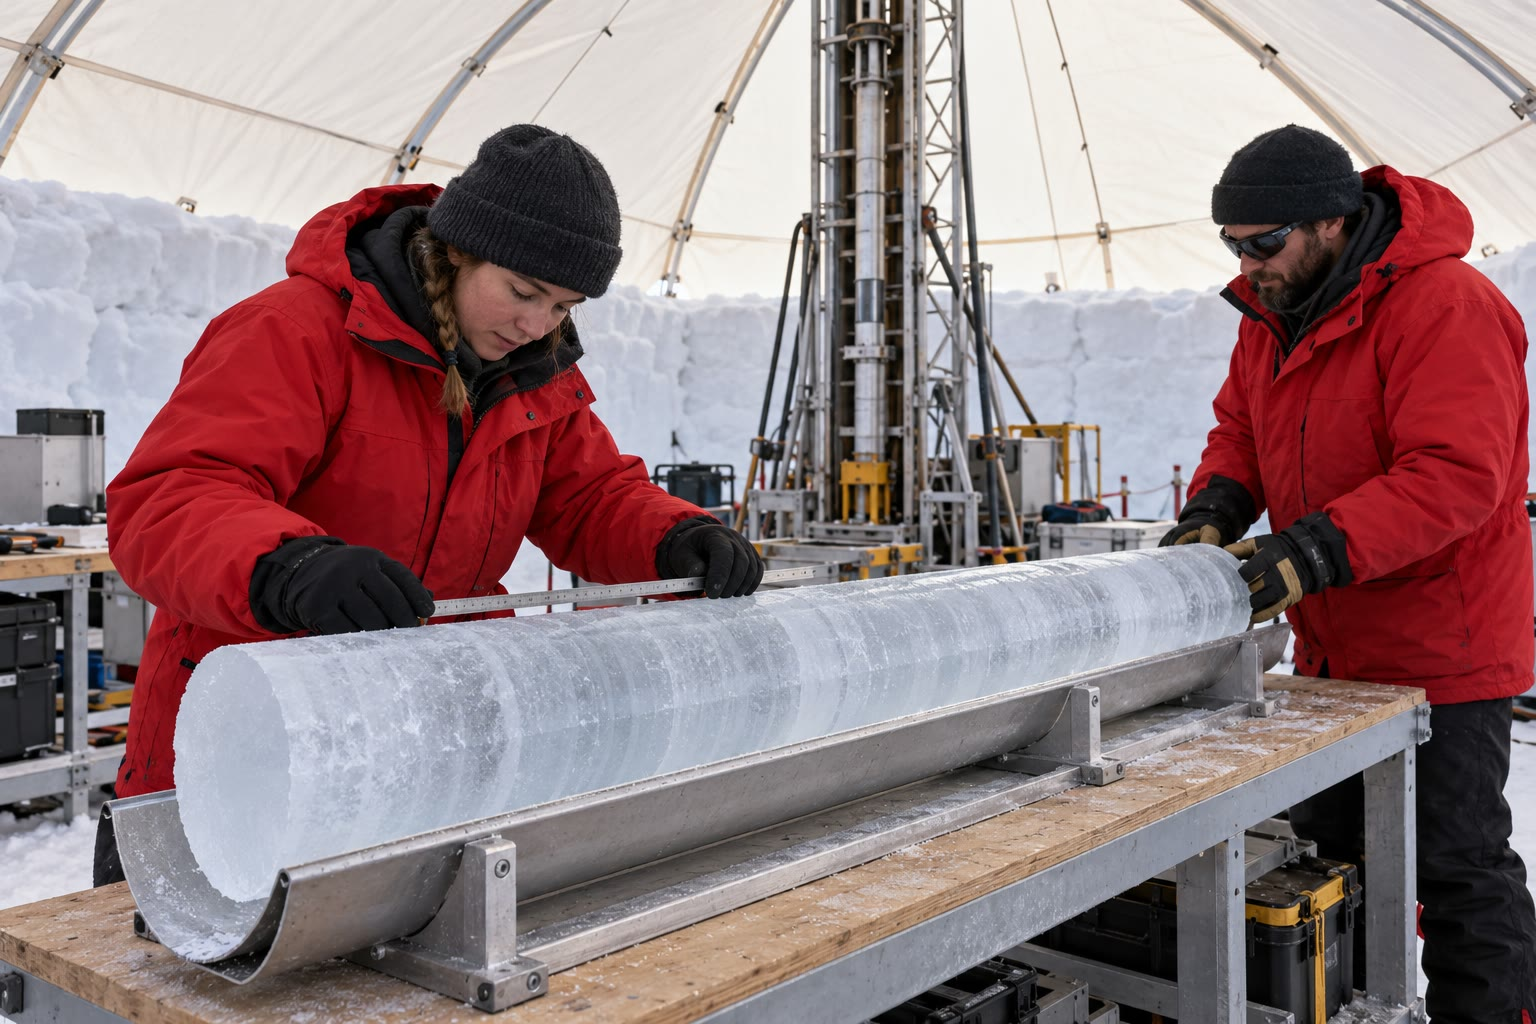
\includegraphics[width=\linewidth]{images/book5/ai/b3-ice-core-tent.jpg}

{\scriptsize قياس لبّ جليدي في حاضنة داخل خيمة حفر على الغطاء
الجليدي، وبرج الحفر في الخلفية (رسم توضيحي مولَّد بالذكاء الاصطناعي).}
\end{minipage}
\end{inthelab}

\section{التمارين}

\begin{exercise}[$\star$]\label{exo:b3:stable-isotopes:1}
لدينا كالسيت له $\delta^{18}\mathrm O = \qty{30.5}{\permil}$، والماء الذي نما منه
\qty{-2.1}{\permil}، وكلاهما مقاس على VSMOW. احسب $\alpha$، $1000\ln\alpha$
و$\Delta$. ما مقدار التباعد بين الاثنين الأخيرين؟
\end{exercise}

\begin{exercise}[$\star$]\label{exo:b3:stable-isotopes:2}
لمحطة ساحلية في خطوط العرض العالية متوسّط درجة حرارة سنوية قدره
\qty{-25}{\celsius}. باستخدام العلاقات الواردة في الفصل لمثل هذه المحطات،
توقّع $\delta^{18}\mathrm O$، و$\delta\mathrm D$ \omterm{def:b3:stable-isotopes:d-excess}{وفائض الدوتيريوم}
لهطول تلك المحطة.
\end{exercise}
% ledger: dansgaard64:effects

\begin{exercise}[$\star$]\label{exo:b3:stable-isotopes:3}
في حوض ما، لدى الكربونات $\delta^{13}\mathrm C = \qty{+1.0}{\permil}$، وللمادة
العضوية \qty{-26.0}{\permil}. مع مدخلات عند \qty{-5}{\permil}، احسب
$f_{\mathrm{org}}$.
\end{exercise}
% ledger: planavsky22:forg

\begin{exercise}[$\star$]\label{exo:b3:stable-isotopes:4}
لصدفة ذراعيّة الأرجل $\Delta_{47} = \qty{0.600}{\permil}$. باستخدام معايرة
الفصل، عند أيّ درجة حرارة نمت؟
\end{exercise}
% ledger: isogeochem:d47

\begin{exercise}[$\star\star$]\label{exo:b3:stable-isotopes:5}
يغادر البخار المحيط عند $\delta^{18}\mathrm O = \qty{-13}{\permil}$ ويتساقط
مطرًا بثابت $\alpha = 1.0100$. ما الكسر المتبقّي منه عندما
يبلغ البخار \qty{-33}{\permil}؟ ما قيمة $\delta^{18}\mathrm O$ للمطر
عندئذٍ؟
\end{exercise}
% ledger: white13c9:rayleigh

\begin{exercise}[$\star\star$]\label{exo:b3:stable-isotopes:6}
يُقارن الثلج عند \qty{-40}{\permil} بماء المحيط عند 0. احسب $\alpha$،
$1000\ln\alpha$، $1000(\alpha - 1)$ و$\Delta$ بينهما. أيّ من
تقريبات القضية يفشل، وبأيّ مقدار؟
\end{exercise}

\begin{exercise}[$\star\star$]\label{exo:b3:stable-isotopes:7}
لدى الفورامينيفيرا $\delta^{18}\mathrm O = \qty{+1.50}{\permil}$ مقاسة على VPDB، ونمت في
ماء عند \qty{0.00}{\permil} على VSMOW. احسب درجة حرارة نموّها بطريقة
الفصل، وكم يغيّرها خطأ قدره \qty{0.1}{\permil} في
قيمة الماء.
\end{exercise}
% ledger: isogeochem:ko97

\begin{exercise}[$\star\star$]\label{exo:b3:stable-isotopes:8}
يتغيّر المكدّس القاعي بمقدار \qty{1.77}{\permil} من الوقت الحاضر إلى آخر
عصر جليدي أقصى. استبعد حصّة حجم الجليد المحسوبة في الفصل،
وحوّل الباقي إلى تغيّر في درجة حرارة مياه الأعماق، مستعملًا ميل
معايرة الكالسيت قرب \qty{2}{\celsius}.
\end{exercise}
% ledger: data:lr04, white13c9:ice-volume, isogeochem:ko97

\begin{exercise}[$\star\star$]\label{exo:b3:stable-isotopes:9}
لدى البيريت $\delta^{34}\mathrm S = \qty{10.0}{\permil}$ و$\delta^{33}\mathrm S =
\qty{8.2}{\permil}$. احسب $\Delta^{33}\mathrm S$. ماذا يخبرنا ذلك عن
الغلاف الجوي عند تكوّن البيريت؟
\end{exercise}
% ledger: white13c9:s-mif

\begin{exercise}[$\star\star\star$]\label{exo:b3:stable-isotopes:10}
في التكاثف ذي النظام المغلق، يبقى البخار وكلّ المكثّف المتكوّن
معًا في حالة توازن. بيّن أنّ البخار عندئذٍ له $R_v/R_{v,0} = 1/[f +
\alpha(1 - f)]$، وقارنه \omterm{prop:b3:stable-isotopes:rayleigh-distillation}{بتقطير رايلي} من أجل $f = 0.2$
و$\alpha = 1.01$.
\end{exercise}

\begin{exercise}[$\star\star\star$]\label{exo:b3:stable-isotopes:11}
انطلاقًا من التقدير بأنّ \qty{2000}{Gt} من كربون الميثان عند
\qty{-60}{\permil} يُزيح كربون التبادل بمقدار \qty{-2.5}{\permil}،
فأوجد كتلة الخزّان المستنتجة، مع $\delta_0 = 0$. وبهذه الكتلة، كم
كربونًا عضويًا عند \qty{-25}{\permil} يُعطي الإزاحة نفسها؟ قارن
بالمدى المنشور.
\end{exercise}
% ledger: dickens11:petm

\begin{exercise}[$\star\star\star$]\label{exo:b3:stable-isotopes:12}
بيّن أنّه على مسار التبريد، فإنّ $\mathrm d\delta_v/\mathrm dT = (\alpha - 1)(1000 +
\delta_v)\,\mathrm d\ln e_s/\mathrm dT$. عند \qty{-20}{\celsius}، حيث
يملك بخار نموذج الفصل $\delta^{18}\mathrm O = \qty{-49.1}{\permil}$
ويعطي منحنى التسامي $\mathrm d\ln e_s/\mathrm dT =
\qty{0.0960}{K^{-1}}$، احسب هذا الميل.
\end{exercise}
% ledger: gkinis14:alpha-ice, iapws:melt-subl

\section{مسألة: رحلة قطرة مطر إلى دوم إلسه}

\begin{problem}[{مسألة نهاية الأسبوع --- نظائر الثلج على امتداد
مسار مُتخيَّل، ودرجة حرارة قديمة، وانحراف نظائر الكربون}]\label{pb:b3:stable-isotopes:1}
تغادر كتلة هوائية حافة غطاء جليدي مُتخيَّل عند \qty{0}{\celsius}
ومعها بخار قيمته $\delta^{18}\mathrm O = \qty{-20.0}{\permil}$ و$\delta\mathrm D =
\qty{-150}{\permil}$، وتبرد عند ضغط ثابت مع تقدّمها نحو الداخل.
يتكوّن الثلج في محطة الساحل عند \qty{-10}{\celsius}، وفي ميدواي عند
\qty{-20}{\celsius} وفي دوم إلسه عند \qty{-30}{\celsius}، عندما
يكون كسر البخار المتبقّي هو $f = 0.425$، $0.169$ و$0.0622$. استخدم معاملات تجزّؤ الجليد--البخار
الواردة في الفصل، ثابتةً على كلّ مرحلة عند قيمتها في درجة الحرارة
المتوسّطة لتلك المرحلة.
% ledger: gkinis14:alpha-ice, iapws:melt-subl, dansgaard64:effects, isogeochem:ko97, isogeochem:d47, white13c9:ice-volume, data:lr04, planavsky22:forg, dickens11:petm

\medskip\noindent\textbf{الجزء الأول --- التقطير.}
\begin{enumerate}
\item احسب $\alpha^{18}$ و$\alpha^{\mathrm D}$ عند $-5$، $-10$، $-15$، $-20$،
$-25$ و\qty{-30}{\celsius} (خمسة أرقام معنوية للأكسجين، وأربعة
للدوتيريوم).
\item احسب $\delta^{18}\mathrm O$ للبخار عند وصوله إلى محطة الساحل.
\item احسب القيمة نفسها لثلج محطة الساحل.
\item كرّر الحساب لميدواي (نسبة المرحلة من $f$ هي $0.169/0.425$).
\item كرّر الحساب لدوم إلسه.
\item ما الكسر من الأكسجين-18 الأصلي للبخار الذي ما زال موجودًا
في الهواء عند دوم إلسه؟
\end{enumerate}

\medskip\noindent\textbf{الجزء الثاني --- درجة الحرارة والدوتيريوم.}
\begin{enumerate}[resume]
\item احسب ميل $\delta^{18}\mathrm O$ للثلج مقابل
درجة حرارة التكاثف من الساحل إلى دوم إيلس.
\item أيُّ متوسط سنوي لدرجة حرارة السطح تُسنده علاقة
محطات غرينلاند إلى ثلج دوم إيلس؟ لماذا يمكن أن يختلف عن
\qty{-30}{\celsius}؟
\item احسب $\delta\mathrm D$ للثلج في المحطات الثلاث بالطريقة نفسها.
\item احسب \omterm{def:b3:stable-isotopes:d-excess}{فائض الدوتيريوم} فيها. كيف يتغيّر نحو الداخل؟
\item هل يقع ثلج دوم إيلس على خط المياه المطرية؟ ماذا يُغفل النموذج
الذي يتضمّنه تكوّن الثلج الحقيقي؟
\end{enumerate}

\medskip\noindent\textbf{الجزء الثالث --- منخربية قبالة الساحل.} قلبٌ رسوبيّ قبالة الساحل يُعطي
منخربيات قاعية بقيمة \qty{3.25}{\permil}
VPDB عند القمة، و\qty{5.02}{\permil} عند أقصى تجلّد أخير؛ ماءُ القاع
\qty{0.00}{\permil} VSMOW اليوم.
\begin{enumerate}[resume]
\item احسب درجة حرارة ماء القاع الحالية باستخدام
معايرة الكالسيت.
\item احسب درجة الحرارة الجليدية بافتراض بقاء الماء دون تغيّر. هل
النتيجة ممكنة؟
\item صحّح ماء العصر الجليدي لهبوط مستوى سطح البحر بمقدار \qty{125}{m} وأعِد
الحساب. ما مقدار التبرّد الجليدي لماء القاع؟
\item احسب $\Delta_{47}$ المتوقّع عند الدرجتين
والفرق بينهما.
\item لماذا لا يحتاج مقياس الحرارة \omterm{def:b3:stable-isotopes:clumped}{بالنظائر المتكتّلة} إلى تركيب
الماء؟
\end{enumerate}

\medskip\noindent\textbf{الجزء الرابع --- \omterm{def:b3:stable-isotopes:cie}{انحراف نظائر الكربون}.} وفي عمق أكبر من القلب،
تتقطّع كربونات بقيمة \qty{+0.5}{\permil} بانحراف وجيز بمقدار
\qty{-3.0}{\permil}.
\begin{enumerate}[resume]
\item قبل الانحراف، بافتراض $\delta_{\mathrm{in}} = \qty{-5}{\permil}$
و$\Delta_B = \qty{-28}{\permil}$، احسب $f_{\mathrm{org}}$.
\item خذ الخزّان الوارد في التمرين 11، \qty{46000}{Gt} عند 0. كم من الكربون
يحتاج إليه الانحراف إذا كان المصدر هو الميثان عند \qty{-60}{\permil}؟
\item وإذا كان كربونًا عضويًّا عند \qty{-25}{\permil}؟
\item وإذا كان كربون الوشاح عند \qty{-5}{\permil}؟
\item أيّ ملاحظة في القلب نفسه قد تساعد على الاختيار بين
المصادر؟
\item اذكر $\delta^{18}\mathrm O$ للثلج المتساقط في دوم إيلس.
\end{enumerate}
\end{problem}
